\documentclass[10pt]{beamer}

\usetheme[progressbar=frametitle]{metropolis}
\usepackage{appendixnumberbeamer}

\usepackage{booktabs}
\usepackage[scale=2]{ccicons}

\usepackage{tcolorbox}
\definecolor{darkred}{RGB}{173,34,48}

\usepackage{pgfplots}
\usepgfplotslibrary{dateplot}
\usepackage{tikz}
\usetikzlibrary{snakes}
\usetikzlibrary{decorations}
%\usepackage{xeCJK} %导入中文包
%\setCJKmainfont{SimHei} %中文字体采用黑体  Microsoft YaHei

%\usepackage{pgfplots}
%\usepgfplotslibrary{dateplot}
%\usepackage{tikz}
\usetikzlibrary{shapes.geometric}
%\usetikzlibrary{decorations.markings}
\usetikzlibrary{calc,decorations.markings}
\usepackage{xspace}
\newcommand{\themename}{\textbf{\textsc{metropolis}}\xspace}
\usepackage{xcolor}
	\definecolor{limegreen}{rgb}{0.2, 0.8, 0.2}
\definecolor{nicegreen}{RGB}{102,252,102}
\definecolor{mediumturquoise}{rgb}{0.28, 0.82, 0.8}
\definecolor{oceanboatblue}{rgb}{0.0, 0.47, 0.75}
\definecolor{darkred}{rgb}{0.675,0,0.2}

\newcommand{\dif}{\mathrm{d}}
\newcommand{\me}{\mathrm{e}}
%\newcommand{\mi}{\mathrm{i}}


%================================================================================================================
\newcommand{\fwbox}[2]{\text{\makebox[#1][c]{$\hspace{-150pt}\displaystyle#2\hspace{-150pt}$}}}
\newcommand{\fwboxL}[2]{\text{\makebox[#1][l]{$#2$}}}
\newcommand{\fwboxR}[2]{\text{\makebox[#1][r]{$#2$}}}
\newcommand{\bigger}[1]{\raisebox{-0.95pt}{\scalebox{1.25}{$#1$}}}
\newcommand{\Bigger}[1]{\raisebox{-2.25pt}{\scalebox{1.75}{$#1$}}}
\renewcommand{\Bar}{\overline}
\renewcommand{\tilde}{\widetilde}
\newcommand{\eq}[1]{\vspace{-0.5pt}\begin{equation}\hspace{0pt}#1\hspace{-0pt}\vspace{-0.5pt}\end{equation}}
\newcommand{\fig}[2]{\vcenter{\includegraphics[scale=#1]{#2}}}
\newcommand{\mi}{\raisebox{0.75pt}{\scalebox{0.75}{$\hspace{-1pt}\,-\,\hspace{-0.75pt}$}}}
\newcommand{\pl}{\raisebox{0.75pt}{\scalebox{0.75}{$\hspace{-1pt}\,+\,\hspace{-0.75pt}$}}}
\newcommand{\ab}[1]{\langle #1\rangle}
\newcommand{\equivR}{\fwbox{14.5pt}{\hspace{-0pt}\fwboxR{0pt}{\raisebox{0.47pt}{\hspace{1.25pt}:\hspace{-4pt}}}=\fwboxL{0pt}{}}}
\newcommand{\equivL}{\fwbox{14.5pt}{\fwboxR{0pt}{}=\fwboxL{0pt}{\raisebox{0.47pt}{\hspace{-4pt}:\hspace{1.25pt}}}}}
\renewcommand{\u}[2]{(\hspace{-0.5pt}#1;\hspace{-1.5pt}#2\hspace{-0.5pt})}
\newcommand{\proj}[1]{\raisebox{1.75pt}{\big[}\hspace{-0.75pt}#1\hspace{-0.75pt}\raisebox{1.75pt}{\big]}}
\renewcommand{\r}[1]{\mathfrak{A}\hspace{-0.75pt}(\hspace{-1pt}{\color{hred}#1\hspace{-1pt}})}
\newcommand{\rb}[2]{(\hspace{-1pt}{\color{hblue}#1}\hspace{-1pt})^c_{\fwboxL{4.5pt}{#2}}}
\newcommand{\amp}[1]{\mathfrak{A}_{{\color{hred}#1}}}
\newcommand{\f}[1]{\mathfrak{#1}}
\newcommand{\Zeta}[1]{\zeta_#1}
\newcommand{\Li}[2]{\hspace{1pt}\mathrm{Li}_{#1}(#2)}

\newcommand{\polyalpha}{\rho}
\newcommand{\polybeta}{\sigma}


\definecolor{hblue}{rgb}{0,0,0.575}
\definecolor{hred}{rgb}{0.575,0.0,0.225}
\definecolor{hteal}{rgb}{0.0,0.545,0.7451}
\definecolor{optLegColour}{rgb}{0.5,0.5,0.5}



\def\figScale{0.835}\def\edgeLen{1*\figScale}\def\fScale{\small}\def\legLen{\edgeLen*0.65}\def\labelDist{\legLen*1.45}\def\lineThickness{(1pt)}\def\dotSize{(\figScale*10)}\def\ampSize{(1*\figScale*10pt)}\def\legSpread{5}\def\extLegLen{0.75*0.75*\figScale}
\tikzset{ddot/.style={fill=black,circle,minimum size=0.35*\dotSize,inner sep=0}}
\tikzset{int/.style={black,line width=\lineThickness,line cap=round,rounded corners=0.5pt}}\tikzset{ext/.style={black,line width=\lineThickness,line cap=round}}\tikzset{bdot/.style={fill=black,circle,minimum size=0.45*\ampSize,inner sep=0}}\tikzset{wdot/.style={draw=black,line width=\lineThickness,fill=white,circle,minimum size=0.50*\ampSize,inner sep=0}}
\newcommand{\leg}[3]{\draw[ext] #1--($#1+(#2:\legLen)$);\node at ($#1+(#2:\labelDist)$)[]{{\fScale #3}};}
\newcommand{\optLeg}[2]{\coordinate (aa0) at #1;\coordinate (aa5) at ($#1+(#2+\legSpread*3:\extLegLen)$);\coordinate (bb5) at ($#1+(#2-\legSpread*3:\extLegLen)$);\coordinate (aa1) at ($(aa0)!0.4!(aa5)$);\coordinate (aa2) at ($(aa0)!0.55!(aa5)$);\coordinate (aa3) at ($(aa0)!0.7!(aa5)$);\coordinate (aa4) at ($(aa0)!0.85!(aa5)$);\coordinate (bb1) at ($(aa0)!0.4!(bb5)$);\coordinate (bb2) at ($(aa0)!0.55!(bb5)$);\coordinate (bb3) at ($(aa0)!0.7!(bb5)$);\coordinate (bb4) at ($(aa0)!0.85!(bb5)$);\fill[optLegColour] (aa0)--(aa1)--(bb1)--(aa0);\fill[optLegColour] (aa2)--(aa3)--(bb3)--(bb2)--(aa2);\fill[optLegColour] (aa4)--(aa5)--(bb5)--(bb4)--(aa4);}

\newcommand{\octagonk}{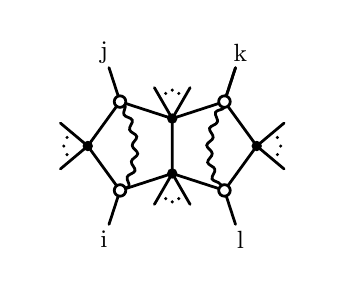
\begin{tikzpicture}[scale=\figScale,baseline=-2.45]\useasboundingbox ($(-7.9/3*\figScale,-1.8)$) rectangle ($(7.9/3*\figScale,1.8)$);\draw[int,line width=0.1,red,draw=none] ($(-7.5/3*\figScale,-1.5)$) rectangle ($(7.5/3*\figScale,1.5)$);\coordinate(v1) at ($(0,0)+(90:\edgeLen/2)$);\coordinate(v2)at($(v1)+(18:\edgeLen)$);\coordinate(v3)at($(v2)+(18-72:\edgeLen)$);\coordinate(v4)at($(v3)+(18-2*72:\edgeLen)$);\coordinate(v5)at($(v4)+(18-3*72:\edgeLen)$);\coordinate(v6)at($(v5)+(198-0*72:\edgeLen)$);\coordinate(v7)at($(v6)+(198-1*72:\edgeLen)$);\coordinate(v8)at($(v7)+(198-2*72:\edgeLen)$);
\draw[int](v1)--(v2)--(v3)--(v4)--(v5)--(v6)--(v7)--(v8)--(v1);\draw[int](v1)--(v5);\leg{(v2)}{72}{k};
\leg{(v1)}{60}{};\leg{(v1)}{120}{};
\leg{(v2)}{72}{};
\leg{(v5)}{-60}{};
\leg{(v5)}{-120}{};
\leg{(v3)}{40}{\!};
\leg{(v3)}{-40}{\!};
\leg{(v7)}{140}{\!};
\leg{(v7)}{-140}{\!};
\node[fill=black,circle,minimum size=0.15*\dotSize,inner sep=0] at (-1.65,0) {};
\node[fill=black,circle,minimum size=0.15*\dotSize,inner sep=0] at (-1.6,0.13) {};
\node[fill=black,circle,minimum size=0.15*\dotSize,inner sep=0] at (-1.6,-0.13) {};
\node[fill=black,circle,minimum size=0.15*\dotSize,inner sep=0] at (1.65,0) {};
\node[fill=black,circle,minimum size=0.15*\dotSize,inner sep=0] at (1.6,0.13) {};
\node[fill=black,circle,minimum size=0.15*\dotSize,inner sep=0] at (1.6,-0.13) {};
\node[fill=black,circle,minimum size=0.15*\dotSize,inner sep=0] at (0,0.85) {};
\node[fill=black,circle,minimum size=0.15*\dotSize,inner sep=0] at (0.1,0.80) {};
\node[fill=black,circle,minimum size=0.15*\dotSize,inner sep=0] at (-0.1,0.80) {};
\node[fill=black,circle,minimum size=0.15*\dotSize,inner sep=0] at (0,-0.85) {};
\node[fill=black,circle,minimum size=0.15*\dotSize,inner sep=0] at (0.1,-0.80) {};
\node[fill=black,circle,minimum size=0.15*\dotSize,inner sep=0] at (-0.1,-0.80) {};
\draw[decorate, decoration=snake, segment length=6pt,segment amplitude=1pt,black,line width=\lineThickness] (v8) to[out=-60,in=60] (v6);
\draw[decorate, decoration=snake, segment length=6pt,segment amplitude=1pt,black,line width=\lineThickness] (v2)to[out=-120,in=120](v4);
\leg{(v4)}{72-2*72}{l};\leg{(v6)}{252-0*72}{i};\leg{(v8)}{252-2*72}{j};\foreach\a in {1,3,5,7}{\node at (v\a) [bdot]{};};\foreach\a in {2,4,6,8}{\node at (v\a) [wdot]{};};
% \node at ($(\edgeLen/1.4,0)$) []{$N_1$};\node at ($(-\edgeLen/1.4,0)$) []{$N_1$};
\end{tikzpicture}}
\newcommand{\octagonkPrime}{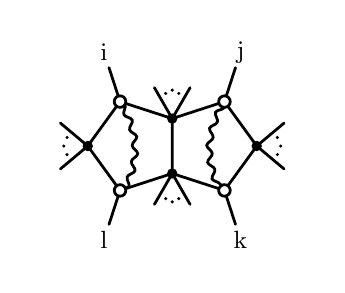
\begin{tikzpicture}[scale=\figScale,baseline=-2.45]\useasboundingbox ($(-7.9/3*\figScale,-1.8)$) rectangle ($(7.9/3*\figScale,1.8)$);\draw[int,line width=0.1,red,draw=none] ($(-7.5/3*\figScale,-1.5)$) rectangle ($(7.5/3*\figScale,1.5)$);\coordinate(v1) at ($(0,0)+(90:\edgeLen/2)$);\coordinate(v2)at($(v1)+(18:\edgeLen)$);\coordinate(v3)at($(v2)+(18-72:\edgeLen)$);\coordinate(v4)at($(v3)+(18-2*72:\edgeLen)$);\coordinate(v5)at($(v4)+(18-3*72:\edgeLen)$);\coordinate(v6)at($(v5)+(198-0*72:\edgeLen)$);\coordinate(v7)at($(v6)+(198-1*72:\edgeLen)$);\coordinate(v8)at($(v7)+(198-2*72:\edgeLen)$);
\draw[int](v1)--(v2)--(v3)--(v4)--(v5)--(v6)--(v7)--(v8)--(v1);\draw[int](v1)--(v5);\leg{(v1)}{60}{};\leg{(v1)}{120}{};
\node[fill=black,circle,minimum size=0.15*\dotSize,inner sep=0] at (-1.65,0) {};
\node[fill=black,circle,minimum size=0.15*\dotSize,inner sep=0] at (-1.6,0.13) {};
\node[fill=black,circle,minimum size=0.15*\dotSize,inner sep=0] at (-1.6,-0.13) {};
\node[fill=black,circle,minimum size=0.15*\dotSize,inner sep=0] at (1.65,0) {};
\node[fill=black,circle,minimum size=0.15*\dotSize,inner sep=0] at (1.6,0.13) {};
\node[fill=black,circle,minimum size=0.15*\dotSize,inner sep=0] at (1.6,-0.13) {};
\node[fill=black,circle,minimum size=0.15*\dotSize,inner sep=0] at (0,0.85) {};
\node[fill=black,circle,minimum size=0.15*\dotSize,inner sep=0] at (0.1,0.80) {};
\node[fill=black,circle,minimum size=0.15*\dotSize,inner sep=0] at (-0.1,0.80) {};
\node[fill=black,circle,minimum size=0.15*\dotSize,inner sep=0] at (0,-0.85) {};
\node[fill=black,circle,minimum size=0.15*\dotSize,inner sep=0] at (0.1,-0.80) {};
\node[fill=black,circle,minimum size=0.15*\dotSize,inner sep=0] at (-0.1,-0.80) {};
\leg{(v2)}{72}{j};
\leg{(v5)}{-60}{};
\leg{(v5)}{-120}{};
\leg{(v3)}{40}{\!};
\leg{(v3)}{-40}{\!};
\leg{(v7)}{140}{\!};
\leg{(v7)}{-140}{\!};
\draw[decorate, decoration=snake, segment length=6pt,segment amplitude=1pt,black,line width=\lineThickness] (v8) to[out=-60,in=60] (v6);
\draw[decorate, decoration=snake, segment length=6pt,segment amplitude=1pt,black,line width=\lineThickness] (v2)to[out=-120,in=120](v4);
\leg{(v4)}{72-2*72}{k};\leg{(v6)}{252-0*72}{l};\leg{(v8)}{252-2*72}{i};\foreach\a in {1,3,5,7}{\node at (v\a) [bdot]{};};\foreach\a in {2,4,6,8}{\node at (v\a) [wdot]{};};
% \node at ($(\edgeLen/1.4,0)$) []{$N_1$};\node at ($(-\edgeLen/1.4,0)$) []{$N_1$};
\end{tikzpicture}}
\newcommand{\mhvInt}{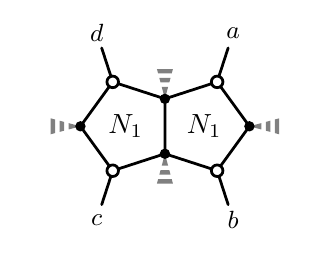
\begin{tikzpicture}[scale=\figScale,baseline=-2.45]\useasboundingbox ($(-7.5/3*\figScale,-1.5)$) rectangle ($(7.5/3*\figScale,1.5)$);\draw[int,line width=0.1,red,draw=none] ($(-7.5/3*\figScale,-1.5)$) rectangle ($(7.5/3*\figScale,1.5)$);\coordinate(v1) at ($(0,0)+(90:\edgeLen/2)$);\coordinate(v2)at($(v1)+(18:\edgeLen)$);\coordinate(v3)at($(v2)+(18-72:\edgeLen)$);\coordinate(v4)at($(v3)+(18-2*72:\edgeLen)$);\coordinate(v5)at($(v4)+(18-3*72:\edgeLen)$);\coordinate(v6)at($(v5)+(198-0*72:\edgeLen)$);\coordinate(v7)at($(v6)+(198-1*72:\edgeLen)$);\coordinate(v8)at($(v7)+(198-2*72:\edgeLen)$);
\draw[int](v1)--(v2)--(v3)--(v4)--(v5)--(v6)--(v7)--(v8)--(v1);\draw[int](v1)--(v5);\optLeg{(v1)}{90};\leg{(v2)}{72}{$a$};\optLeg{(v3)}{72-1*72};\leg{(v4)}{72-2*72}{$b$};\optLeg{(v5)}{-90};\leg{(v6)}{252-0*72}{$c$};\optLeg{(v7)}{252-1*72};\leg{(v8)}{252-2*72}{$d$};\foreach\a in {1,3,5,7}{\node at (v\a) [bdot]{};};\foreach\a in {2,4,6,8}{\node at (v\a) [wdot]{};};
\node at ($(\edgeLen/1.4,0)$) []{$N_1$};\node at ($(-\edgeLen/1.4,0)$) []{$N_1$};
\end{tikzpicture}}


\title{Algebraic letters and NMHV last entry conditions from $\bar{Q}$-equation}
\subtitle{\scriptsize Based on oncoming and recent works with Song He and Zhenjie Li}
% \date{\today}
%\date{}
\author{Chi Zhang}
\institute{Institute of Theoretical Physics, CAS}
 %\titlegraphic{\includegraphics[height=1.0cm]{logo.png}\hfill}

\begin{document}

\maketitle




\section{Last entry conditions}


\begin{frame}[t]{N$^{2}$MHV Yangian invariants}


The N$^{2}$MHV Yangian invariants have already been classified. {\footnotesize[\textcolor{darkred}{Arkani-Hamed, Bourjaily, Cachazo, Goncharov, Postnikov, Trnka}]}

They are 
\begin{columns}
  \column{0.5\textwidth}
  \tiny
  \begin{align*}
    Y^{(2)}_1 &= [1,2,(23)\cap (456), (234) \cap (56) , 6] [2,3,4,5,6] \\
    \nonumber
    Y^{(2)}_2 &= [1,2,(34) \cap (567), (345) \cap (67), 7] [3,4,5,6,7] \\
    \nonumber
    Y^{(2)}_3 &= [1,2,3,(345) \cap (67), 7] [3,4,5,6,7] \\
    \nonumber
    Y^{(2)}_4 &= [1,2,3,(456) \cap (78), 8] [4,5,6,7,8] \\
    \nonumber
    Y^{(2)}_5 &= [1,2,3,4,8] [4,5,6,7,8] \\
    \nonumber
    Y^{(2)}_6 &= [1,2,3,(45) \cap (678), 8] [4,5,6,7,8] \\
    Y^{(2)}_7 &= [1,2,3,(45) \cap (678), (456) \cap (78)] [4,5,6,7,8]
  \end{align*}
  \column{0.5\textwidth}
  \tiny
  \begin{align*}
    Y^{(2)}_8 &= [1,2,3,4,(456) \cap (78)] [4,5,6,7,8] \\
    \nonumber
    Y^{(2)}_9 &= [1,2,3,4,9] [5,6,7,8,9] \\
    \nonumber
    Y^{(2)}_{10}&=[1,2,3,4,(567) \cap (89)] [5,6,7,8,9] \\
    \nonumber
    Y^{(2)}_{11}&=[1,2,3,4,(56) \cap (789)] [5,6,7,8,9] \\
    \nonumber
    Y^{(2)}_{12}&= \varphi 
    [1,2,3,(45) \cap (789) , (46) \cap (789)] [(45) \cap (123), (46) \cap (123), 7,8,9] \\
    Y^{(2)}_{13}&=[1,2,3,4,5][6,7,8,9,10] \\
    Y^{(2)}_{14}&=\psi [A,1,2,3,4][B,5,6,7,8]
    \nonumber
  \end{align*}
\end{columns}
  where
  \begin{align*}
  (i j) \cap (k l m ) = \mathcal{Z}_i \langle j\, k\, l\, m \rangle - \mathcal{Z}_j \langle i\, k \, l\, m \rangle
  \end{align*}

\end{frame}

\begin{frame}[t]{NMHV last entry conditions}
  For N$^{2}$MHV yangian invariants, this operation gives three kinds of last entries \\
\footnotesize{
1.
\begin{flalign*}
   [i\,j\,k\,l\,m] \bar{Q}\log\frac{\langle\bar{n}a\rangle}{\langle\bar{n}b\rangle}
\end{flalign*}
2.
\begin{align*}
  &[1\,i_{1}\,i_{2}\,i_{3}\,i_{4}]\,\bar{Q}\log\frac{\langle 1(n{-}1\,n)(i_{1}\,i_{2})(i_{3}\,i_{4})\rangle}{\langle\bar{n}i_{1}\rangle\langle1i_{2}i_{3}i_{4}\rangle} \:,  \quad 
  [i_{1}\,i_{2}\,i_{3}\,i_{4}\,n{-}1]\,\bar{Q}\log\frac{\langle n{-}1(n\,1)(i_{1}\,i_{2})(i_{3}\,i_{4})\rangle}{\langle\bar{n}i_{1}\rangle\langle n{-}1\,i_{2}i_{3}i_{4}\rangle} \\
  &[i_{1}\,i_{2}\,i_{3}\,i_{4}\,n]\,\bar{Q}\log\frac{\langle n(1\,n{-1})(i_{1}\,i_{2})(i_{3}\,i_{4})\rangle}{\langle\bar{n}i_{1}\rangle\langle n\,i_{2}i_{3}i_{4}\rangle} \quad\text{with} \,1<i_{1}<i_{2}<i_{3}<i_{4}<n{-}1 \nonumber
\end{align*}
where $\langle a(bc)(de)(fg)\rangle :=\langle abde\rangle\langle acfg\rangle -\langle acde\rangle\langle abfg\rangle$}

3. \begin{equation*}
  [i_{1}\,i_{2}\,i_{3}\,i_{4}\,i_{5}]\,\bar{Q}\log\frac{\langle \bar{n}(i_{1}i_{2})\cap(i_{3}i_{4}i_{5})\rangle }{\langle \bar{n}i_{1}\rangle \langle i_{2}i_{3}i_{4}i_{5}\rangle } \:, \:\: [i_{1}\,i_{2}\,i_{3}\,i_{4}\,i_{5}]\,\bar{Q}\log\frac{\langle \bar{n}(i_{1}i_{2}i_{3})\cap(i_{4}i_{5})\rangle }{\langle \bar{n}i_{1}\rangle \langle i_{2}i_{3}i_{4}i_{5}\rangle } \:,
\end{equation*}
with $1<i_{1}<i_{2}<i_{3}<i_{4}<i_{5}<n$
\end{frame}


% \begin{frame}[fragile,t]{Why octagon?}
  
% The surprise simplicity of $6$ and $7$-point amplitudes:
% \begin{itemize}
%   \item  The symbol alphabet for six-particle kinematics consists of 9 letters, which correspond to cluster algebra $G(4,6)$
%   \item  The symbol alphabet for seven-particle kinematics consists of 42 letters, which correspond to cluster algebra $G(4,7)$
% \end{itemize}
% With further physical constrains on the iterated structure of cuts, the 6-point amplitude has been determined through 7 loop for MHV and 6 loop for NMHV, the 7-point amplitude has been determined through 4 loop for both MHV and NMHV. [\textcolor{darkred}{Caron-Huot, Dixon, Drummond,\ldots}]

% For more than seven particles, symbol alphabets are not well understood
% \begin{itemize}
%   \item  $G(4,n\geq 8)$ are infinite-type cluster algebras.
%   \item algebraic roots appear in symbol letters even at one-loop in N$^{2}$MHV
%   amplitudes
% \end{itemize}

% \end{frame}

\section{Algebraic letters and words in two-loop NMHV amplitudes}

\begin{frame}[t]{Input}
To compute the 2-loop NMHV $n$ point BDS-normalized amplitude, we need the input of the one-loop N$^{2}$MHV BDS-normalized amplitude $R_{n+1,2}^{(1)}$, which can be obtained from the chiral/scalar box expansion {\footnotesize[\textcolor{darkred}{Bourjaily, Caron-Huot, Trnka}]}:
\begin{equation*}
  R_{n+1,2}^{(1)} =\sum_{a<b<c<d} (f_{a,b,c,d}-R_{n+1,2}^{\text{tree}} f_{a,b,c,d}^{\text{MHV}})\mathcal{I}_{a,b,c,d}^{\text{fin}}
\end{equation*}
where
\begin{itemize}
  \item $f_{a,b,c,d}$ are linear combinations of N$^{2}$MHV yangian invariants
  \item $f_{a,b,c,d}^{\text{MHV}}$ are either 1 or 0
  \item $\mathcal{I}_{a,b,c,d}^{fin}$ denote the finite part of DCI-regulated box integrals
\end{itemize}

\end{frame}

\begin{frame}[t]{Four-mass box}
The most generic term in box expansion:\\[5pt]
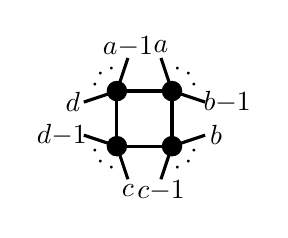
\begin{tikzpicture}[baseline={([yshift=-.5ex]current bounding box.center)},scale=0.7]
  \node[fill=black,circle,draw=black, inner sep=0pt,minimum size=7pt] at (-2,0) {};
  \node[fill=black,circle,draw=black, inner sep=0pt,minimum size=7pt] at (-2,-1) {};
  \node[fill=black,circle,draw=black, inner sep=0pt,minimum size=7pt] at (-1,-1) {};
  \node[fill=black,circle,draw=black, inner sep=0pt,minimum size=7pt] at (-1,0) {};
  \draw[line width=0.4mm] (-2,0) -- (-2,-1) -- (-1,-1) -- (-1,0) -- cycle;
  \draw[line width=0.4mm] (-2.6,-0.8) -- (-2,-1);
  \draw[line width=0.4mm] (-2,-1) -- (-1.8,-1.6);
  \draw[line width=0.4mm] (-1,-1) -- (-0.4,-0.8);
  \draw[line width=0.4mm] (-1,-1) -- (-1.2,-1.6);
  \draw[line width=0.4mm] (-2.6,-0.2) -- (-2,0);
  \draw[line width=0.4mm] (-1.8,0.6) -- (-2,0);
  \draw[line width=0.4mm] (-1.2,0.6) -- (-1,0);
  \draw[line width=0.4mm] (-1,0) -- (-0.4,-0.2);
  \node at (-1.2,0.8) {$a$};
  \node at (0,-0.2) {$b{-}1$};
  \node at (-0.2,-0.8) {$b$};
  \node at (-1.2,-1.8) {$c{-}1$};
  \node at (-1.8,-1.8) {$c$};
  \node at (-3,-0.8) {$d{-}1$};
  \node at (-2.8,-0.2) {$d$};
  \node at (-1.8,0.8) {$a{-}1$};
  \node at (-2.4,0.1) {$\cdot$};
  \node at (-2.3,0.3) {$\cdot$};
  \node at (-2.1,0.4) {$\cdot$};
  \node at (-0.9,-1.4) {$\cdot$};
  \node at (-0.7,-1.3) {$\cdot$};
  \node at (-0.6,-1.1) {$\cdot$};
  \node at (-0.6,0.1) {$\cdot$};
  \node at (-0.7,0.3) {$\cdot$};
  \node at (-0.9,0.4) {$\cdot$};
  \node at (-2.4,-1.1) {$\cdot$};
  \node at (-2.3,-1.3) {$\cdot$};
  \node at (-2.1,-1.4) {$\cdot$};
\end{tikzpicture}
$ \scriptsize \displaystyle
  \begin{cases}\displaystyle
      u=\displaystyle\frac{x_{ad}^{2}x_{bc}^{2}}{x_{ac}^{2}x_{bd}^{2}},\quad v=\displaystyle\frac{x_{ab}^{2}x_{cd}^{2}}{x_{ac}^{2}x_{bd}^{2}}, \quad 
      \Delta_{abcd} =\sqrt{(1{-}u{-}v)^{2}-4uv}   \\[12pt]  
      z_{a,b,c,d}=\frac{1}{2}(1+u-v+\Delta), \: 
      \bar{z}_{a,b,c,d}=\frac{1}{2}(1+u-v+\Delta),
  \end{cases}
$

For such a box, 
\begin{align*}
  f_{a,b,c,d} &= \sum_{\pm}\frac{1-u-v\pm\Delta}{2\Delta}[\alpha_{\pm},b{-1},b,c-1,c][\delta_{\pm},d{-1},d,a{-}1,a] \\
  \mathcal{I}_{a,b,c,d}^{\text{fin}}&= \operatorname{Li}_{2}(z)-\operatorname{Li}_{2}(\bar{z})+\frac{1}{2}\log(z\bar{z})\log{\frac{1-z}{1-\bar{z}}}
\end{align*}
where $\alpha_{\pm}$ and $\delta_{\pm}$ are two solutions of Schubert problem $\alpha=(a{-}1 \,a)\cap (d\,d{-}1\,\gamma)$, $\gamma=(c{-}1 \,c)\cap (b\,b{-}1\,\alpha)$

\uncover<2>{The square root will disappear when one mass corner become massless, {\it e.g.} $b=a{+1}$}
\end{frame}

\begin{frame}{Rationalize the square root $\Delta$}

Only $f_{a,b,c,n+1}$ and $f_{1,b,c,n}$ survive under the $\dif^{2\vert3}Z_{n+1}$ integration,

since
\[
\Delta_{1,b,c,n} \xrightarrow[]{\mathcal{Z}_{n+1}\vert\vert \mathcal{Z}_{n}} 1-\frac{x_{1b}^{2}x_{cn}^{2}}{x_{1c}^{2}x_{bn}^{2}}
\]


% Under the collinear limit of $\mathcal{Z}_{n+1}\vert\vert \mathcal{Z}_{n}$, some $\Delta$'s become algebraic functions $\Delta(\tau)$ of $\tau$.

% \begin{itemize}
%   \setlength{\itemsep}{20pt}
%   \item Perform $\tau$-integral for four-mass box coefficients $f_{a,b,c,d}$ is difficult due to the appearance of square root $\Delta$.
%   \item However, $\Delta(\tau)$ can be rationlized by a variable substitution, since $\Delta^{2}$ is only a quadratic polynomial of $\tau$.
%   \item 
%   This is just the classic problem to find a rational parameterization of a quadratic curve $y^{2}=x^{2}+ax+b$.
% \end{itemize}

\end{frame}





\begin{frame}{Algebraic letters of two-loop NMHV amplitudes}

\footnotesize{
  1-D $\tau$-integrals for these four masses introduce new algebraic letters
  \begin{equation*}
    \mathcal{X}_{a,b,c,d}^{\ast}:=\frac{(x^{\ast}_{a,b,c,d}+1)^{-1}-\bar{z}_{d,a,b,c}}{(x^{\ast}_{a,b,c,d}+1)^{-1}-z_{d,a,b,c}}\:, \qquad     
    \widetilde{\mathcal{X}}_{a,b,c,d}^{\ast}:=\frac{(x^{\ast}_{a,b,c,d-1}+1)^{-1}-z
    _{d,a,b,c}}{(x^{\ast}_{a,b,c,d-1}+1)^{-1}-\bar{z}_{d,a,b,c}}
\end{equation*}
with 6 choices $a{-}1,a,b{-}1,b,c{-}1,c$ of the superscript, where
\begin{align*}
    & x^{a}_{a,b,c,d}=\frac{\langle\overline{d} (c{-}1\,c)\cap(a\,b{-}1\,b) \rangle}{\langle \overline{d}\,a\rangle \langle b{-}1\,b\,c{-}1\,c\rangle} \:, \qquad x^{a-1}_{a,b,c,d}= x^{a}_{a,b,c,d}\vert_{a\leftrightarrow a{-}1}\\
   %  x_{a}=\frac{\langle \bar{n} (c-1\,c)\cap(a\,b{-}1\,b)\rangle}{\langle\bar{n}\,a\rangle \langle b{-}1\,b\,c{-}1\,c \rangle} \\
    &x_{a,b,c,d}^{b}=\frac{\langle \overline{d} (c{-}1\,c)\cap (a{-}1\,a\,b)\rangle}{\langle \overline{d} (a{-}1\,a)\cap(b\,c{-}1\,c)\rangle} \:, \qquad x^{b-1}_{a,b,c,d}= x^{b}_{a,b,c,d}\vert_{b\leftrightarrow b{-}1} \\
    &x_{a,b,c,d}^{c}=\frac{\langle \overline{d}\,c\rangle\langle a{-}1\,a\,b{-}1\,b\rangle}{\langle \overline{d}(a{-}1\,a)\cap(b{-}1\,b\,c)\rangle} \:, \qquad x^{c-1}_{a,b,c,d}= x^{c}_{a,b,c,d}\vert_{c\leftrightarrow c{-}1}  \nonumber  
\end{align*}
Note that $\mathcal{X}_{a,b,c,d}^{\ast}$, $\mathcal{X}_{b,c,d,a}^{\ast}$, $\mathcal{X}_{c,d,a,b}^{\ast}$ and $\mathcal{X}_{d,a,b,c}^{\ast}$ involve the same square root $\Delta_{a,b,c,d}$

}

\end{frame}

\begin{frame}{Counting}
  Na\"{i}vely, there are would be $12\times 4 +2 =50$ letters associated with the same $\Delta_{a,b,c,d}$. 

  However, some degeneracy happens when some mass corners only involve 2 particles, for example
  \[
    \mathcal{X}_{d+2,b,c,d}^{d+1}=\frac{\bar{z}_{d,d+2,b,c}}{z_{d,d+2,b,c}}\:,\qquad 
    \widetilde{\mathcal{X}}_{a,b,d-2,c}^{d-2}=\frac{1-z_{d,a,b,d-2}}{1-\bar{z}_{d,a,b,d-2}} \:.
  \]
  This leave us $50-2m$ algebraic letters associated with the same $\Delta$ where 
  \[
  m= \text{ the number of corners that contain only two particles}
  \]
  These $\mathcal{X}$'s and $\widetilde{\mathcal{X}}$'s, together with $z/\bar{z}$ and $(1-z)/(1-\bar{z})$ give a cyclic and reflection invariant set of algebraic letters %whose logarithms are invariant up to a sign under the cyclic rotation $i\to i{+1}$ and the reflection $i\to n{-}i{+}1$. 
  
\end{frame}


\begin{frame}{Multiplicative relations among algebraic letters}
\footnotesize{
33 multiplicative relations:
  \begin{gather*}
    \frac{\mathcal{X}_{a,b,c,d}^{a-1}}{\mathcal{X}_{a,b,c,d}^{a}} =\frac{\mathcal{X}_{d,a,b,c}^{a}}{\mathcal{X}_{d,a,b,c}^{a-1}}\:,\quad \frac{\mathcal{X}_{d,a,b,c}^{a-1}}{\mathcal{X}_{d,a,b,c}^{a}} =\frac{\mathcal{X}_{c,d,a,b}^{a}}{\mathcal{X}_{c,d,a,b}^{a-1}}\:, \nonumber \\
    \frac{\widetilde{\mathcal{X}}_{a,b,c,d}^{a-1}}{\widetilde{\mathcal{X}}_{a,b,c,d}^{a}} =\frac{\widetilde{\mathcal{X}}_{d,a,b,c}^{a}}{\widetilde{\mathcal{X}}_{d,a,b,c}^{a-1}}\:,\quad \frac{\widetilde{\mathcal{X}}_{d,a,b,c}^{a-1}}{\widetilde{\mathcal{X}}_{d,a,b,c}^{a}} =\frac{\widetilde{\mathcal{X}}_{c,d,a,b}^{a}}{\widetilde{\mathcal{X}}_{c,d,a,b}^{a-1}}  \:,\\
    \frac{\mathcal{X}_{a,b,c,d}^{a-1}}{\mathcal{X}_{a,b,c,d}^{a}}=\frac{\widetilde{\mathcal{X}}_{c,d,a,b}^{a}}{\widetilde{\mathcal{X}}_{c,d,a,b}^{a-1}} \:,\quad \frac{\mathcal{X}_{a,b,c,d}^{a}}{\mathcal{X}_{a,b,c,d}^{b}}=\frac{\widetilde{\mathcal{X}}_{a,b,c,d}^{b}}{\widetilde{\mathcal{X}}_{a,b,c,d}^{a}}\:,\qquad 
    \frac{\mathcal{X}_{a,b,c,d}^{b}}{\mathcal{X}_{a,b,c,d}^{c}}=\frac{\widetilde{\mathcal{X}}_{a,b,c,d}^{c}}{\widetilde{\mathcal{X}}_{a,b,c,d}^{b}} \nonumber
    \end{gather*}
    and 21 images under the rotations of $a\to b\to c\to d\to a$, 
    \begin{gather*}
      \frac{\mathcal{X}_{a,b,c,d}^{a}\mathcal{X}_{b,c,d,a}^{d}\mathcal{X}_{c,d,a,b}^{d}\mathcal{X}_{d,a,b,c}^{a}}{\mathcal{X}_{a,b,c,d}^{b}\mathcal{X}_{b,c,d,a}^{c}\mathcal{X}_{c,d,a,b}^{c}\mathcal{X}_{d,a,b,c}^{b}} =1 \:, \\
      \frac{\mathcal{X}_{a,b,c,d}^{a}\mathcal{X}_{b,c,d,a}^{d}\mathcal{X}_{d,a,b,c}^{a}}{\mathcal{X}_{a,b,c,d}^{c}\mathcal{X}_{b,c,d,a}^{c}\mathcal{X}_{d,a,b,c}^{d}} =1 \:,\quad 
      \frac{\mathcal{X}_{b,c,d,a}^{b}\mathcal{X}_{c,d,a,b}^{a}\mathcal{X}_{d,a,b,c}^{a}}{\mathcal{X}_{b,c,d,a}^{c}\mathcal{X}_{c,d,a,d}^{c}\mathcal{X}_{d,a,b,c}^{b}} =1 \:, \nonumber
  \end{gather*}
  \begin{equation*} %\label{productrelation3}
      \frac{\mathcal{X}_{c,d,a,b}^{a}\mathcal{X}_{d,a,b,c}^{a}}{\mathcal{X}_{c,d,a,b}^{d}\mathcal{X}_{d,a,b,c}^{d}} =\frac{z_{a,b,c,d}}{\bar{z}_{a,b,c,d}} \:,\quad 
      \frac{\mathcal{X}_{b,c,d,a}^{c}\mathcal{X}_{c,d,a,b}^{c}}{\mathcal{X}_{b,c,d,a}^{d}\mathcal{X}_{c,d,a,b}^{d}} = \frac{1-z_{a,b,c,d}}{1-\bar{z}_{a,b,c,d}} \:.
  \end{equation*}
}   

Taking these relations into account:
\[
\text{number of multiplicatively independent algebraic letters} = 17-2m
\]
\end{frame}


\begin{frame}{Two kinds of cuts}
  
  The algebraic letters can be rewritten as $(a\pm \sqrt{a^{2}-4b})$.\\
  $(a,b)$ are polynomials of Pl\"{u}cker coordinates. \\
  Such letters indicate two kinds of cuts:
  \begin{itemize}
    \item One arise from the discriminant $a^{2}-4b$.
    \item The other arise from $b\to0$ which is the same as the cut of $\log b$. 
  \end{itemize}
That is, $b$ must belong to the alphabet of \alert{rational letters}:\\
For example {\footnotesize{
\begin{equation*}
  \begin{aligned}
  \bigl|(x^{c}_{a,b,c,d}+1)^{-1}-\bar{z}_{d,a,b,c}\bigr|^{2}&\propto\langle c(A)(B)(D)\rangle\langle(A) \cap(\overline{d}) B(C) \cap(\overline{d})\rangle\langle A B\rangle \:,\\
  \bigl|(x^{b}_{a,b,c,d}+1)^{-1}-\bar{z}_{d,a,b,c}\bigr|^{2}&\propto \langle b(A)(C)(D)\rangle\langle(A) \cap(\overline{d}) B(C) \cap(\overline{d})\rangle \:, \\
  \bigl|(x^{a}_{a,b,c,d}+1)^{-1}-\bar{z}_{d,a,b,c}\bigr|^{2}&\propto \langle a(B)(C)(D)\rangle\langle(A) \cap(\overline{d}) B(C) \cap(\overline{d})\rangle\langle B C\rangle \:,
  \end{aligned} 
\end{equation*}
}}
here $A=(a{-1}\,a)$, $B=(b{-}1\,b)$, $C=(c{-}1\,c)$, $D=(d{-}1\,d)$
\end{frame}

\begin{frame}{Algebraic Words}
 For non-degenerate $\mathcal{X}_{a,b,c,d}^{\ast}$'s, then the algebraic words reads
  \begin{align*}
      &\quad \mathcal{S}(I_{a,b,c,d})\otimes \mathcal{X}_{a,b,c,d}^{c-1}\otimes x_{a,b,c,d}^{c-1} \,[a{-}1\,a\,b{-1}\,b\,c-1] \nonumber \\
      &-\mathcal{S}(I_{a,b,c,d})\otimes \mathcal{X}_{a,b,c,d}^{c}\otimes x_{a,b,c,d}^{c} \,[a{-}1\,a\,b{-1}\,b\,c] \nonumber \\
      &+ \mathcal{S}(I_{a,b,c,d})\otimes \mathcal{X}_{a,b,c,d}^{b-1}\otimes x_{a,b,c,d}^{b-1} \,[a{-}1\,a\,b{-1}\,c-1\,c] \nonumber \\
      &-\mathcal{S}(I_{a,b,c,d})\otimes \mathcal{X}_{a,b,c,d}^{b}\otimes x_{a,b,c,d}^{c} \,[a{-}1\,a\,b\,c{-1}\,c] \nonumber \\
      &+\mathcal{S}(I_{a,b,c,d})\otimes \mathcal{X}_{a,b,c,d}^{a-1}\otimes x_{a,b,c,d}^{a-1} \,[a{-}1\,b{-1}\,b\,c-1\,c] \nonumber \\
      &-\mathcal{S}(I_{a,b,c,d})\otimes \mathcal{X}_{a,b,c,d}^{a}\otimes x_{a,b,c,d}^{a} \,[a\,b{-1}\,b\,c{-}1\,c]  \:,\label{Xalgebraicword}
  \end{align*}
likewise for $\tilde{\mathcal{X}}$. Recall that 
\begin{equation*}
  \mathcal{X}^{\ast}:=\frac{(x^{\ast}+1)^{-1}-\bar{z}}{(x^{\ast}+1)^{-1}-z}\:, 
\end{equation*}
\end{frame}

\begin{frame}{A class of special components}
 The $\chi_{i}\chi_{j}\chi_{k}\chi_{l}$ component with $i,j,k,l$ nonadjacent
  \begin{itemize}
    \item first show up at the two-loop order,
    \item \alert{completely free} of algebraic letters,
    \item correspond to the difference of double-pentagon integrals {\footnotesize [\textcolor{darkred}{Arkani-Hamed, Bourjaily, Cachazo, Trnka}]}
  \end{itemize}
\vspace{-2mm}
\begin{equation*}
  \octagonk-\octagonkPrime,
\end{equation*}
each of which depend on {\alert{many}} algebraic roots.{\footnotesize [\textcolor{darkred}{Bourjaily, McLeod, Vergu, Volk, von Hippel, Wilhelm}]}

%\only<2>{The symbol size $\sim$ $2.8\times 10^{4}$ terms}
\end{frame}

%\section{Outlook}

\begin{frame}{Outlook}

\begin{itemize}
  \item Octagons and algebraic letters at three-loop MHV and two-loop N$^{2}$MHV.
  \item The connection to cluster algebra, tropical Grassmannian
  \item $\bar{Q}$ equations for individual integral and other theories.
\end{itemize}


\end{frame}

\section*{Thank You}


\appendix
\iffalse
\only<2> { \item For $k=1$, it's non-trivial, since   
\begin{align*}
\bar{Q} [1,2,3,4,5]\log\frac{\langle1234\rangle}{\langle2345\rangle} &= [1,2,3,4,5]\bar{Q} \log\frac{\langle1234\rangle}{\langle2345\rangle} \\
  &= (\bar{3})_{a} [1,2,3,4,5]\frac{\langle 1234\rangle\chi^{A}_{5}+\text{cyclic}}{\langle2345\rangle\langle 2341\rangle}
\end{align*}}
one example:
\begin{align*}
  Y_{1}^{(2)} \propto \bar{Q}\log u\bar{Q}\log v\bar{Q}\log w
\end{align*}
% where $u=\frac{\langle 1234\rangle\langle 4561\rangle}{\langle 1245\rangle\langle 3461\rangle}$, $v=\frac{\langle 3456\rangle\langle 6123\rangle}{\langle 3461\rangle\langle 5623\rangle}$, $w=\frac{\langle 5612 \rangle\langle 1234\rangle}{\langle 5623\rangle\langle 1245\rangle}$
then it is easy to see that 
\[
\bar{Q}\bigl(Y_{1}^{2}F(u,v,w)\bigr) =0 
\]
for any function $F$ of $u,v,w$.
\fi

\begin{frame}{The kernel of $\bar{Q}$}
  When k=1,
  \begin{align*}
    \bar{Q} \biggl([1,2,3,4,5]\log\frac{\langle1234\rangle}{\langle2345\rangle}\biggr) &= [1,2,3,4,5]\bar{Q} \log\frac{\langle1234\rangle}{\langle2345\rangle} \\
      &= (\bar{3})_{a} [1,2,3,4,5]\frac{\langle 1234\rangle\chi^{A}_{5}+\text{cyclic}}{\langle2345\rangle\langle 2341\rangle}
    \end{align*}
    When k=2, it's easy to show 
    \begin{align*}
      Y_{1}^{(2)}=\frac{\delta^{0\vert 4}(\langle 1234\rangle\chi_{5}\chi_{6}+\text{cyclic})}{\langle 1234\rangle\cdots \langle 6123\rangle} \propto \bar{Q}\log u\bar{Q}\log v\bar{Q}\log w
    \end{align*}
    then 
    \begin{equation*}
    \bar{Q}\bigl(Y_{1}^{(2)}F(u,v,w)\bigr)=0
    \end{equation*}
\end{frame}


\begin{frame}{Outline of derivation of $\bar{Q}$-equation} 

By using chiral Lagrangian insertion {\footnotesize[\textcolor{darkred}{Caron-Huot}]}, one can show  
\begin{equation*}
  \bar{Q}_{\dot{\alpha}}^{A}\langle W_{n,k}\rangle \propto \oint \dif x_{\dot{\alpha}\alpha} 
  \langle (\psi^{A}+F\theta^{A}+\cdots)^{\alpha} W_{n,k}\rangle
\end{equation*}
To obtain the $\bar{Q}$-equation, there are two powerful facts:
\begin{itemize}
  \item The fermion insertion is the unique twist-one excitation with the quantum numbers of $\bar{Q}$.
  \item Its expectation value can be extracted from any object having a nonzero overlap with it in the OPE limit. {\footnotesize[\textcolor{darkred}{ Alday, Gaiotto, Maldacena, Sever, Vieira}]}
\end{itemize}
$\langle W_{n+1,k+1}\rangle$ has a nonzero overlap with $\bar{Q}_{\dot{\alpha}}^{A}\langle W_{n,k}\rangle$ under the colliner limit, while $\int \dif^{2\vert 3} \mathcal{Z}_{n+1}$ has the same quantum number as $\bar{Q}$, 
\begin{equation*}
  \bar{Q}_{\dot{\alpha}}^{A}\langle W_{n,k}\rangle \propto \int \dif^{2\vert 3} \mathcal{Z}_{n+1} \langle W_{n+1,k+1}\rangle 
\end{equation*}

\end{frame} 

\iffalse
\begin{frame}[fragile]{Example: Rationalize a Circle}
  Key point: find the rational points!


  A unit circle defined by 
  \[
   y^{2}=1-x^{2}  
  \]
  own (0,1) as its rational point, then we can intersert $y=t(x-1)$ into this quadratic curve:
  \begin{align*}
    t^{2}(x-1)^{2} &=1-x^{2} \\
                 \Rightarrow x &= \frac{t^{2}-1}{t^{2}+1} \\
                 \Rightarrow y&=t(x-1)= -\frac{2t}{1+t^{2}}
  \end{align*}
\end{frame}


\begin{frame}{Example: Rationalize $f_{2,4,6,9}$}
  Let's focus on the octagon (n=8), for which nine 9-point four-mass boxes is needed. It is easy to see only 
  \begin{equation*}
    f_{2,4,7,9},\qquad f_{2,5,7,9},\qquad f_{2,4,6,9},\qquad f_{3,5,7,9} 
  \end{equation*}
  can potentially contribute square root. Where $f_{2,4,6,9}$ and $f_{3,5,7,9}$ indeed contribute two square roots $\Delta_{1,3,5,7}$ and $\Delta_{2,4,6,8}$ respectively.
 
  $\Delta_{2,4,6,9}(\tau)$ owns $\tau=\infty$ as its rational point. Thus, we can find the following substitution
  \begin{equation*}
    \tau=\frac{\rho (t-z_{2,4,6,8})(t-\bar{z}_{2,4,6,8})}{t-\sigma}
  \end{equation*} 
  where $\rho$ and $\sigma$ are some cross ratios of Pl\"{u}cker coordinates.
 
  The square root in $z_{2,4,6,8}$ enters the final result via the limit of integration $\int_{0}^{\infty} \dif\tau\to \int_{z}^{\infty}\dif t \, \dif \tau/\dif t$
 \end{frame}

\fi
\end{document}
